\documentclass{article}
\usepackage[T1]{fontenc}
\usepackage{lmodern}
\usepackage{amssymb,latexsym,amsmath,dk,dkenv}
\usepackage{tikz}
\usepgflibrary{shapes}
\usetikzlibrary{arrows,automata,backgrounds}
\usepackage{bbm}

\usepackage[all]{xy}
\usepackage{algorithm}
\usepackage[noend]{algpseudocode}

\DeclareFontFamily{U}{mathb}{\hyphenchar\font45}
\DeclareFontShape{U}{mathb}{m}{n}{<5> <6> <7> <8> <9> <10> gen * mathb <10.95> mathb10 <12> <14.4> <17.28> <20.74> <24.88> mathb12}{}
\DeclareSymbolFont{mathb}{U}{mathb}{m}{n}
\DeclareMathSymbol\fsmash\mathbin{mathb}{"0C}

\newcommand\rsem[1]{[#1]}
\newcommand\lsem[1]{L\den{#1}}
\newcommand\cset[1]{\{#1\}}
\newcommand\Rel{\kw{Rel}}
\newcommand\KL{\kw{Kl}}
\newcommand\KLP{\ensuremath{\KL\,\PP}} 
\newcommand\lam[2]{\lambda{#1}\kern1pt.\kern1pt{#2}}
\newcommand\nf[1]{#1^{\mathrm{nf}}}
\newcommand\CA{\ensuremath{P}}
\newcommand\At{\ensuremath{\mathit{At}}}
\newcommand\cseq[2]{\pseq{\pseq{#1}\cdots}{#2}}
\renewcommand\smash{\mathrel{\diamond}}
\newcommand\ssum{\mathop{\textstyle\sum}}
\newcommand\sbigcup{\mathop{\textstyle\bigcup}}
\newcommand\pdup{\mathop{\mathsf{dup}}}
\newcommand\One{\mathbf{1}}
\newcommand\Two{\mathbf{2}}
\newcommand\Exp{\mathsf{Exp}}
\newcommand\bval[1]{[#1]}
\renewcommand\star{^{\textstyle *}}
\newcommand\id{\mathsf{id}}
\newcommand\NetHKC[2]{\texttt{NetKATEquiv}(#1,#2)}
\newcommand\pair[2]{\langle #1,#2\rangle}
\renewcommand\powerset[1]{\Two^{#1}}
\newcommand\JI{\At\cdot(P\cdot\pdup)\star\cdot P}
\newcommand\setJI{2^{\At\cdot P\cdot(\pdup\cdot P)^{\scriptstyle *}}}
\newcommand\funJI{(2^{\At \cdot P})^{(P\cdot\pdup)^{\scriptstyle *}}}

\begin{document}

\section{NetKAT}

\subsection*{Language Semantics}

We identify sets in $2^Q$ with their characteristic functions $Q\fun 2$, writing $x\in A$ and $A(x)=1$ interchangeably.

Let $\setJI$ be the set of join-irreducibles. For $A,B\in\setJI$, define
\begin{gather*}
A+B = A\cup B \qquad
0 = \emptyset \qquad
1 = \id = \set{\alpha p_\alpha}{\alpha\in\At}\\
A\smash B = \set{yz}{\exists q\ yq\in A,\ \alpha_qz\in B} \qquad
A\star = \sbigcup_n A^n \qquad
\bar A = \id\setminus A
\end{gather*}
This is a KAT. The canonical interpretation $G:\Exp\fun\setJI$ of regular expressions over $P\cup\At\cup\cset\pdup$ is:
\begin{gather*}
G(p) = \set{\alpha p}{\alpha\in\At} \qquad
G(b) = \set{\alpha p_\alpha}{\alpha\leq b} \qquad
G(\pdup) = \set{\alpha p_\alpha\pdup p_\alpha}{\alpha\in\At}\\
G(e_1+e_2) = G(e_1)\cup G(e_2) \qquad
G(e_1e_2) = G(e_1)\smash G(e_2) \qquad
G(e\star) = \sbigcup_n G(e^n)\\
G(0) = \emptyset \qquad
G(1) = \set{\alpha p_\alpha}{\alpha\in\At} \qquad
G(\bar b) = G(1) \setminus G(b)
\end{gather*}

Define
\begin{gather*}
\bval\phi = \begin{cases}
1, & \phi\\
0, & \neg\phi
\end{cases}
\end{gather*}
In terms of characteristic functions,
\begin{align*}
(A\smash B)(x) &= \ssum_{x=yz}\bval{\exists q\ yq\in A\wedge\alpha_qz\in B}\\
&= \ssum_{x=yz}\ssum_q\bval{yq\in A}\cdot\bval{\alpha_qz\in B}\\
&= \ssum_{x=yz}\ssum_q A(yq)\cdot B(\alpha_qz)
\end{align*}
Note that we must have $y\in\At\cdot(P\cdot\pdup)\star$ and $z\in P\cdot(\pdup\cdot P)\star$ for this to be type-correct.

\section{NetKAT Coalgebraically}

Let $\setJI$ be the set of join-irreducibles. Using elementary bicartesian transformations and the Kleene algebra identity $ab\star = ab\star b + a$, we have an isomorphism
\begin{align}
\setJI
%&\cong 2^{\At\cdot P\cdot(\pdup\cdot P)^{\scriptstyle *}\cdot\pdup\cdot P + \At\cdot P}\nonumber\\
&\cong (\setJI)^{\pdup\cdot P} \times 2^{\At\cdot P}\label{eq:isom2}
\end{align}
Under this isomorphism, a set $A\in\setJI$ on the left corresponds to the pair of functions
\begin{align*}
\delta(A)(\pdup p)(x) &= A(x\pdup p) &
\eps(A)(\alpha q) &= A(\alpha q)
\end{align*}
on the right. We will often use the alternative notation
\begin{align*}
\delta_{\pdup p}(A) &= \delta(A)(\pdup p) & \eps_{\alpha p}(A) &= \eps(A)(\alpha p),
\end{align*}
thus
\begin{align*}
\delta_{\pdup p} &: \setJI\fun\setJI & \eps_{\alpha p} &: \setJI\fun 2.
\end{align*}

The isomorphism \eqref{eq:isom2} allows the set $S = \setJI$ to be endowed with a (Moore) automaton structure for the functor $FX = X^{\pdup\cdot P} \times 2^{\At\cdot P}$: 
\begin{align*}
\delta &: S \to S^{\pdup \cdot P} & \eps &: S \to 2^{\At \cdot P} & \pair\delta\eps : S\fun FS.
\end{align*}

The Moore automaton $\pair\delta\eps$ has the special property of being the final coalgebra for the functor $F$, which means that any other Moore automaton of the same type can be uniquely mapped to it via an $F$-coalgebra morphism. We will define a Moore automaton structure
\begin{align*}
\pair DE : \Exp \to \Exp^{\pdup\cdot P} \times 2^{\At\cdot P}
\end{align*}
on the set $\Exp$ of NetKAT expressions, then show that the unique map $G:\Exp\to S$ is precisely the language semantics defined in the original NetKAT paper \cite{netkat}. This will allow us to use coinduction as a proof principle to determine equivalence of NetKAT expressions. 

\begin{lemma}\ 
\begin{enumerate}
\romanize
\item
$\eps(\id) = \id$
\item
$\eps(\ssum_n A_n) = \ssum_n \eps(A_n)$
\item
$\eps(A\smash B) = \eps(A)\smash\eps(B)$
\end{enumerate}
\end{lemma}

\begin{proof}
(i) $\eps_{\alpha p}(\id) = \id(\alpha p) = \bval{\alpha=\alpha_p}$.\\

(ii)
%\begin{align*}
%\eps_{\alpha p}(\sbigcup_n A_n)
%&= \bval{\alpha p\in\sbigcup_n A_n}
%= \ssum_n\bval{\alpha p\in A_n}
%= \ssum_n\eps_{\alpha p}(A_n)
%\end{align*}
%
\begin{align*}
\eps(\ssum_n A_n)(\alpha p)
&= (\ssum_n A_n)(\alpha p)
= \ssum_n A_n(\alpha p)\\
&= \ssum_n \eps(A_n)(\alpha p)
= (\ssum_n\eps(A_n))(\alpha p)
\end{align*}

(iii)
%\begin{align*}
%\eps_{\alpha p}(A\smash B)
%&= \bval{\alpha p\in A\smash B}
%= \bval{\exists q\ \alpha q\in A\meet \alpha_q p\in B}\\
%&= \ssum_q \bval{\alpha q\in A}
%\cdot
%\bval{\alpha_q p\in B}
%= \ssum_q\eps_{\alpha q}(A)\cdot\eps_{\alpha_q p}(B)
%\end{align*}
%
\begin{align*}
\eps(A\smash B)(\alpha p)
&= (A\smash B)(\alpha p)
= \ssum_q\ A(\alpha q)\cdot B(\alpha_qp)\\
&= \ssum_q\eps(A)(\alpha q)\cdot\eps(B)(\alpha_qp)
= (\eps(A)\smash\eps(B))(\alpha p)
\end{align*}
%
%(iv)
%\begin{align*}
%\eps(A\star)(\alpha p)
%&= \eps_{\alpha p}(\id + A\smash A\star)
%= \eps_{\alpha p}(\id) + \ssum_q\eps_{\alpha q}(A)\cdot\eps_{\alpha_q p}(A\star)
%\end{align*}
\end{proof}

\begin{lemma}\ 
\begin{enumerate}
\romanize
\item
$\delta_{\pdup p}(\ssum_n A_n) = \ssum_n \delta_{\pdup p}(A_n)$
\item
$\delta_{\pdup p}(A\smash B) = A\smash\delta_{\pdup p}(B) + \ssum_{q}\delta_{\pdup q}(A)\cdot\eps_{\alpha_qp}(B)$
\end{enumerate}
\end{lemma}

\begin{proof}
(i)
%\begin{align*}
%\delta_{\pdup p}(\sbigcup_n A_n)
%&= \set{x}{x\pdup p\in\sbigcup_n A_n}\\
%&= \sbigcup_n \set{x}{x\pdup p\in A_n}\\
%&= \sbigcup_n \delta_{\pdup p}(A_n)
%\end{align*}
%
\begin{align*}
\delta_{\pdup p}(\ssum_n A_n)(x)
&= (\ssum_n A_n)(x\pdup p)
= \ssum_n A_n(x\pdup p)\\
&= \ssum_n \delta_{\pdup p}(A_n)(x)
\end{align*}

(ii)
%\begin{align*}
%\delta_{\pdup p}(A\smash B)
%&= \delta_{\pdup p}(\set{yz}{\exists q\ yq\in A,\ \alpha_qz\in B})\\
%&= \delta_{\pdup p}(\set{yz}{\exists q\ yq\in A,\ \alpha_qz\in B,\ z\in P})\\
%&\qquad \cup\delta_{\pdup p}(\set{yz}{\exists q\ yq\in A,\ \alpha_qz\in B,\ z\not\in P})\\
%&= \delta_{\pdup p}(\set{yr}{\exists q\ yq\in A,\ \alpha_qr\in B})\\
%&\qquad \cup\delta_{\pdup p}(\set{yw\pdup r}{\exists q\ yq\in A,\ \alpha_qw\pdup r\in B})
%\end{align*}
%
\begin{align*}
\delta_{\pdup p}(A\smash B)(x)
&= (A\smash B)(x\pdup p)
= \ssum_{x\pdup p=yz}\ssum_q A(yq)\cdot B(\alpha_qz)\\
&= \ssum_{x=yz}\ssum_q A(yq)\cdot B(\alpha_qz\pdup p) + \ssum_q A(x\pdup q)\cdot B(\alpha_qp)\\
&= \ssum_{x=yz}\ssum_q A(yq)\cdot\delta_{\pdup p}(B)(\alpha_qz) + \ssum_q \delta_{\pdup q}(A)(x)\cdot\eps_{\alpha_qp}(B)\\
&= (A\smash\delta_{\pdup p}(B))(x) + (\ssum_q \delta_{\pdup q}(A)\cdot\eps_{\alpha_qp}(B))(x)\\
&= (A\smash\delta_{\pdup p}(B) + \ssum_q \delta_{\pdup q}(A)\cdot\eps_{\alpha_qp}(B))(x)\\
\end{align*}
%
%
%and
%\begin{align*}
%& \delta_{\pdup p}(\set{yr}{\exists q\ yq\in A,\ \alpha_qr\in B})\\
%&= \set{x}{x\pdup p\in\set{yr}{\exists q\ yq\in A,\ \alpha_qr\in B}}\\
%&= \set{x}{x\pdup p\in\set{x\pdup p}{\exists q\ x\pdup q\in A,\ \alpha_qp\in B}}\\
%&= \set{x}{\exists q\ x\pdup q\in A,\ \alpha_qp\in B}\\
%&= \set{x}{\exists q\ x\in\delta_{\pdup q}(A),\ \alpha_qp\in B}\\
%&= \sbigcup \set{\delta_{\pdup q}(A)}{\alpha_qp\in B}
%\end{align*}
%
%\begin{align*}
%& \delta_{\pdup p}(\set{yw\pdup r}{\exists q\ yq\in A,\ \alpha_qw\pdup r\in B})\\
%&= \set x{x\pdup p\in\set{yw\pdup r}{\exists q\ yq\in A,\ \alpha_qw\pdup r\in B}}\\
%&= \set{yw}{yw\pdup p\in\set{yw\pdup p}{\exists q\ yq\in A,\ \alpha_qw\pdup p\in B}}\\
%&= \set{yw}{\exists q\ yq\in A,\ \alpha_qw\pdup p\in B}\\
%&= \set{yw}{\exists q\ yq\in A,\ \alpha_qw\in\delta_{\pdup p}\in B}\\
%&= A\smash\delta_{\pdup p}(B)
%\end{align*}
\end{proof}

\subsection*{Syntactic Coalgebra}

\begin{gather*}
E_{\alpha p}(q) = \bval{q = p} \qquad
E_{\alpha p}(b) = \bval{\alpha_p=\alpha\leq b} \qquad
E_{\alpha p}(\pdup) = 0\\
E_{\alpha p}(e_1+e_2) = E_{\alpha p}(e_1)+E_{\alpha p}(e_2) \qquad
E_{\alpha p}(e_1e_2) = \ssum_{q} E_{\alpha q}(e_1)\cdot E_{\alpha_q p}(e_2)\\
E_{\alpha p}(e\star) = \ssum_n E_{\alpha p}(e^n)
\end{gather*}

\begin{gather*}
D_{\pdup p}(q) = 0 \qquad
D_{\pdup p}(b) = 0 \qquad
D_{\pdup p}(\pdup) = \alpha_p\\
D_{\pdup p}(e_1+e_2) = D_{\pdup p}(e_1)+D_{\pdup p}(e_2)\\
D_{\pdup p}(e_1e_2) = e_1\cdot D_{\pdup p}(e_2) + \ssum_{q} D_{\pdup q}(e_1)\cdot E_{\alpha_qp}(e_2)\\
D_{\pdup p}(e\star) = e\star\cdot D_{\pdup p}(e) + \ssum_{q} D_{\pdup q}(e\star)\cdot E_{\alpha_qp}(e)
\end{gather*}

\subsection*{Main Result}

\begin{theorem}\ 
\label{thm:main}
\begin{enumerate}
\romanize
\item
$E_{\alpha p}(e) = \eps_{\alpha p}(G(e))$
\item
$G(D_{\pdup p}(e)) = \delta_{\pdup p}(G(e))$
\end{enumerate}
\end{theorem}

\begin{proof}
(i) By induction on $e$.
\begin{gather*}
E_{\alpha p}(q)
= \bval{q = p}
= \bval{\alpha p\in\set{\beta q}{\beta\in\At}}
= \eps_{\alpha p}(G(q))\\
E_{\alpha p}(b)
= \bval{\alpha=\alpha_p\leq b}
= \bval{\alpha p\in\set{\beta p_\beta}{\beta\leq b}}
= \eps_{\alpha p}(G(b))\\
E_{\alpha p}(\pdup)
= 0
= \bval{\alpha p\in\set{\alpha p_\alpha\pdup p_\alpha}{\alpha\in\At}}
= \eps_{\alpha p}(G(\pdup))
\end{gather*}

\begin{align*}
E_{\alpha p}(e_1+e_2)
&= E_{\alpha p}(e_1)+E_{\alpha p}(e_2)
= \eps_{\alpha p}(G(e_1)) + \eps_{\alpha p}(G(e_2))\\
&= \eps_{\alpha p}(G(e_1)\cup G(e_2)) 
= \eps_{\alpha p}(G(e_1+e_2))
\end{align*}

\begin{align*}
E_{\alpha p}(e_1e_2)
&= \ssum_{q} E_{\alpha q}(e_1)\cdot E_{\alpha_q p}(e_2)
= \ssum_{q} \eps_{\alpha q}(G(e_1))\cdot \eps_{\alpha_q p}(G(e_2))\\
&= \eps_{\alpha p}(G(e_1)\smash G(e_2))
= \eps_{\alpha p}(G(e_1e_2))
\end{align*}

\begin{align*}
E_{\alpha p}(e\star)
&= \ssum_n E_{\alpha p}(e^n)
= \ssum_n \eps_{\alpha p}(G(e^n))\\
&= \eps_{\alpha p}(\sbigcup_n G(e^n))
= \eps_{\alpha p}(G(e\star)).
\end{align*}

(ii) By induction on $e$.
\begin{align*}
G(D_{\pdup p}(q))
&= G(0)
= \emptyset\\
&= \set{x}{x\pdup p\in\set{\beta q}{\beta\in\At}}\\
&= \delta_{\pdup p}(\set{\beta q}{\beta\in\At})
= \delta_{\pdup p}(G(q))
\end{align*}

\begin{align*}
G(D_{\pdup p}(b))
&= G(0)
= \emptyset\\
&= \set{x}{x\pdup p\in\set{\beta p_\beta}{\beta\leq b}}\\
&= \delta_{\pdup p}(\set{\beta p_\beta}{\beta\leq b})
= \delta_{\pdup p}(G(b))
\end{align*}

\begin{align*}
G(D_{\pdup p}(\pdup))
&= G(\alpha_p)
= \cset{\alpha_pp}\\
&= \set{\alpha_pp}{\alpha_pp\pdup p\in\set{\beta p_\beta\pdup p_\beta}{\beta\in\At}}\\
&= \set{x}{x\pdup p\in\set{\beta p_\beta\pdup p_\beta}{\beta\in\At}}\\
&= \delta_{\pdup p}(\set{\beta p_\beta\pdup p_\beta}{\beta\in\At})
= \delta_{\pdup p}(G(\pdup))
\end{align*}

\begin{align*}
G(D_{\pdup p}(e_1+e_2))
&= G(D_{\pdup p}(e_1)+D_{\pdup p}(e_2))
= G(D_{\pdup p}(e_1))\cup G(D_{\pdup p}(e_2))\\
&= \delta_{\pdup p}(G(e_1))\cup\delta_{\pdup p}(G(e_2))
= \delta_{\pdup p}(G(e_1)\cup G(e_2))\\
&= \delta_{\pdup p}(G(e_1+e_2))
\end{align*}

\begin{align*}
G(D_{\pdup p}(e_1e_2))
&= G(e_1\cdot D_{\pdup p}(e_2) + \ssum_{q} D_{\pdup q}(e_1)\cdot E_{\alpha_qp}(e_2))\\
&= G(e_1)\smash G(D_{\pdup p}(e_2)) \cup \sbigcup\set{G(D_{\pdup q}(e_1))}{E_{\alpha_qp}(e_2)=1}\\
&= G(e_1)\smash \delta_{\pdup p}(G(e_2)) \cup \sbigcup\set{\delta_{\pdup q}(G(e_1))}{\alpha_qp\in G(e_2)}\\
&= \delta_{\pdup p}(G(e_1)\smash G(e_2))
= \delta_{\pdup p}(G(e_1e_2))
\end{align*}

The expressions $D_{\pdup p}(e\star)$ are defined by the system
\begin{align}
X_{p} = e\star\cdot D_{\pdup p}(e) + \ssum_{q} X_{q}\cdot E_{\alpha_qp}(e),\quad p\in P.\label{eq:sys}
\end{align}
The expressions $D_{\pdup p}(e\star)$ for $p\in P$ represent the least solution of \eqref{eq:sys}. Thus
%\begin{align*}
%D_{\pdup p}(e\star) = e\star\cdot D_{\pdup p}(e) + \ssum_{q} D_{\pdup q}(e\star)\cdot E_{\alpha_qp}(e)
%\end{align*}
%thus
\begin{align*}
G(D_{\pdup p}(e\star))
&= G(e\star\cdot D_{\pdup p}(e)) \cup G(\ssum_{q} D_{\pdup q}(e\star)\cdot E_{\alpha_qp}(e))\\
&= G(e\star)\smash G(D_{\pdup p}(e)) \cup \sbigcup_q G(D_{\pdup q}(e\star)\cdot E_{\alpha_qp}(e))\\
&= G(e\star)\smash\delta_{\pdup p}(G(e)) \cup \sbigcup \set{G(D_{\pdup q}(e\star))}{\alpha_qp\in G(e)}
\end{align*}
and the $G(D_{\pdup p}(e\star))$ are the least solution of these equations.
We want to show that $\delta_{\pdup p}(G(e\star))$ is also the least solution of the same equations; that is,
\begin{align}
\delta_{\pdup p}(G(e\star))
&= G(e\star)\smash\delta_{\pdup p}(G(e)) \cup \sbigcup \set{\delta_{\pdup q}(G(e\star))}{\alpha_qp\in G(e)}\label{eq:dsol}
\end{align}
and if $X_p$, $p\in P$ is any other solution, then $\delta_{\pdup p}(G(e\star)) \subs X_p$.

For \eqref{eq:dsol}, since $\delta_{\pdup p}(\id) = \emptyset$,
\begin{align*}
\delta_{\pdup p}(G(e\star))
&= \delta_{\pdup p}(G(1+e\star e))\\
&= \delta_{\pdup p}(\id) \cup \delta_{\pdup p}(G(e\star)\smash G(e))\\
&= G(e\star)\smash\delta_{\pdup p}(G(e)) \cup \sbigcup \set{\delta_{\pdup q}(G(e\star))}{\alpha_qp\in G(e)}.
\end{align*}
Now suppose $X_p$, $p\in P$ satisfy \eqref{eq:sys}.
%\begin{align*}
%X_p
%&= G(e\star)\smash\delta_{\pdup p}(G(e)) \cup \sbigcup \set{X_{\pdup q}}{\alpha_qp\in G(e)}
%\end{align*}
Proceeding by induction on $n$,
\begin{align*}
\delta_{\pdup p}(G(e^0))
&= \delta_{\pdup p}(\id)
= \emptyset
\subs X_p\\[1ex]
\delta_{\pdup p}(G(e^{n+1}))
&= \delta_{\pdup p}(G(e^n)\smash G(e))\\
&= G(e^n)\smash\delta_{\pdup p}(G(e)) \cup \sbigcup \set{\delta_{\pdup q}(G(e^n))}{\alpha_qp\in G(e)}\\
&\subs G(e\star)\smash\delta_{\pdup p}(G(e)) \cup \sbigcup \set{X_{\pdup q}}{\alpha_qp\in G(e)}\\
&= X_p
\end{align*}
therefore
\begin{align*}
\delta_{\pdup p}(G(e\star))
&= \delta_{\pdup p}(\sbigcup_n G(e^n))
= \sbigcup_n\delta_{\pdup p}(G(e^n))
\subs X_p.
\end{align*}
\end{proof}

We remark that the system \eqref{eq:sys} is of a very simple form, and it is easy to compute the expressions $D_{\pdup p}(e\star)$ from it. Note that all $E_{\alpha_qp}(e)$ are either 0 or 1. Thus the system is equivalent to a matrix-vector equation $AX + B = X$, where $A$ is a square 0,1-matrix with rows and columns indexed by $P$ such that $A_{pq} = E_{\alpha_qp}(e)$, $X$ is a vector of variables whose $p$th element is $X_p$, and $B$ is a vector of constants whose $p$th element is $e\star\cdot D_{\pdup p}(e)$. The least solution of \eqref{eq:sys} is represented by $A\star B$. The matrix $A\star$ represents the reflexive transitive closure of the binary relation represented by $A$, which can be computed from $A$ in $O(n^2)$ time by depth-first search. We can then take
\begin{align*}
D_{\pdup p}(e\star) &= (A\star B)_p = e\star\cdot\ssum_{A^{\scriptstyle*}_{pq}=1} D_{\pdup q}(e).
\end{align*}

Theorem \ref{thm:main} says that the following diagram commutes:
\begin{center}
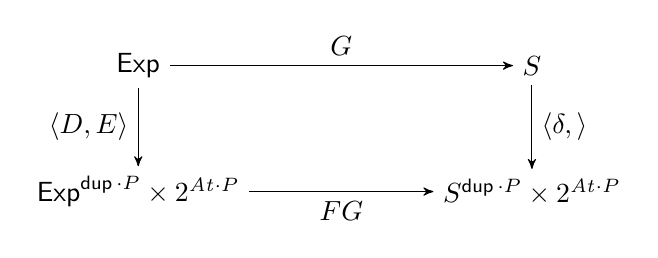
\begin{tikzpicture}[->, >=stealth', node distance=16mm, auto]
  \node (NW) {$\Exp$};
  \node (NE) [right of=NW, node distance=50mm] {$S$};
  \node (SW) [below of=NW] {$\Exp^{\pdup\cdot P}\times 2^{\At\cdot P}$};
  \node (SE) [below of=NE] {$S^{\pdup\cdot P} \times 2^{\At\cdot P}$};
  \path (NW) edge node {$G$} (NE);
  \path (NW) edge node [swap] {$\pair DE$} (SW);
  \path (SW) edge node [swap] {$FG$} (SE);
  \path (NE) edge node {$\pair\delta\eps$} (SE);
\end{tikzpicture}
\end{center}
where $FX = X^{\pdup\cdot P}\times 2^{\At\cdot P}$ with $FG(f,g) = (G\circ f,g)$.

We can now build an automaton $M_e = (S_e, D, E, e)$ with states $S_e\subs S$ obtained by successively applying $D$ starting from $e$, transitions $D$, observations $E$, and start state $e$. This automaton might not be finite, but we can make it  finite by identifying expressions modulo ACI.

\subsection{Decision Procedure}

Given two NetKAT expressions $e_1$ and $e_2$, we build two finite automata $<e_1>$ and $<e_2>$ and then check for their equivalence in the usual way. 

\begin{itemize}
\item When taking derivatives, we can ensure finiteness by taking \emph{Antimirov derivatives} instead and producing a nondeterministic Moore automaton. 
\item We can then for both deterministic and nondeterministic check equivalence up to $+$. This reduces the size of the bisimulation. 
\item We can check equivalence by minimizing both automata using the Brzozowski algorithm for Moore automata and then checking if they are the same. 
\item We could also use position automata. 
\end{itemize}

\newcommand{\todo}{\textsf{todo}}
\renewcommand{\algorithmicrequire}{\textbf{Input:}}
\renewcommand{\algorithmicensure}{\textbf{Output:}}
\renewcommand{\algorithmiccomment}[1]{\hfill$\triangleleft$ {\footnotesize #1}}

\begin{algorithm}
  \caption{Usual bisimulation algorithm for Moore automata
    \label{alg:Moore_naive}}
  \begin{algorithmic}[1]
  \Require Two NetKAT expressions $e_1$ and $e_2$, coalgebra on expressions $E$ and $D$.
  \Ensure Yes/No for equivalence of expressions and a witness (bisimulation).
\Function{NetHKC} {$e_1,e_2$}
\State $R \gets \emptyset$; $\todo \gets \{(e_1,e_2)\}$;\\
 \While{ $\todo$ is not empty} 
     \State extract $(e,f)$ from $\todo$;
      \If{$(e,f)\in (R\cup \todo)/\equiv_{ACI}$} continue; \Comment{Check if (e,f), mod ACI,}\\
     {\footnotesize  \hfill was already in $R\cup \todo$}
      \Else \If {$E(e) \neq E(f)$} return false; \Comment{outputs differ, not bisimilar}
      \Else\ for all { $p\in P$} \Comment{outputs agree, add all derivatives to be checked}
       \State  insert $(D_{p\pdup}(e),D_{p\pdup}(f))$ in $\todo$;
       \EndIf
       \EndIf
\State insert $(e,f)$ in $R$; \Comment{$(e,f)$ has been checked}\\
return true;
\EndFunction
\end{algorithmic}
\end{algorithm}

\begin{remark}
The membership test above, done modulo ACI, is to guarantee that the algorithm above terminates (that the number of pairs added in $R$ is finite). Another weaker check could be done by defining a normal form function that eliminates all duplicates in a sum. This would potentially generate more pairs to be checked but would relieve work in each membership test. 
\end{remark}


\begin{algorithm}
  \caption{Usual bisimulation algorithm for Moore automata with less than ACI
    \label{alg:Moore_naive_2}}
  \begin{algorithmic}[1]
  \Require Two NetKAT expressions $e_1$ and $e_2$, coalgebra on expressions $E$ and $D$.
  \Ensure Yes/No for equivalence of expressions and a witness (bisimulation).
\Function{NetHKC} {$e_1,e_2$}
\State $R \gets \emptyset$; $\todo \gets \{(\text{\sc nf}({e_1}),\text{\sc nf}({e_2}))\}$;\\
 \While{ $\todo$ is not empty} 
     \State extract $(e,f)$ from $\todo$;
      \If{$(e,f)\in R\cup \todo$} continue; \Comment{Check if (e,f) was already in $R\cup \todo$}
      \Else \If {$E(e) \neq E(f)$} return false; \Comment{outputs differ, not bisimilar}
      \Else\ for all { $p\in P$} \Comment{outputs agree, add all derivatives to be checked}
       \State  insert $(\text{\sc nf}(D_{p\pdup}(e)),\text{\sc nf}(D_{p\pdup}(f)))$ in $\todo$;
       \EndIf
       \EndIf
\State insert $(e,f)$ in $R$; \Comment{$(e,f)$ has been checked}\\
return true;
\EndFunction

\Function{nf} {$e$}
\If {$e=e_1+e_2$} 
	\If {$\text{\sc nf}(e_1) = \text{\sc nf}(e_2)$}\ return $\text{\sc nf}(e_1)$ \Else\ return $\text{\sc nf}(e_1) + \text{\sc nf}(e_2)$
	  \EndIf
\Else\ return $e$
  \EndIf
\EndFunction

\end{algorithmic}
\end{algorithm}

Similar to the above, avoiding the use of a normal form, but requiring an extra step of determinization, is to use the analogue of Antimirov derivatives for regular expressions. The derivative of the sum, instead of being the sum of derivatives, is now a set containing the two derivatives. This gives rise to a nondeterministic automaton and, therefore, the equivalence check needs to be done using the subset construction. 

We now define $N \colon \Exp \to \mathcal P(\Exp)^{\pdup \cdot P}$.
\begin{align*}
& N_{p\pdup} \colon \Exp \to \mathcal P(\Exp)  \\
& N_{p\pdup} (q) = \emptyset \\
& N_{p\pdup} (b) = \emptyset \\
& N_{p\pdup} (\pdup) =  \{\alpha_p\}\\
& N_{p\pdup} (e_1+e_2) =  D_{p\pdup}  (e_1) \cup  D_{p\pdup}  (e_2) \\
& N_{p\pdup} (e_1e_2) = D_{p\pdup} (e_1)e_2 \cup E(e_1)D_{p\pdup} (e_2) \\
& N_{p\pdup} (e^*) = D_{p\pdup} (e)e^* \cup E(e)D_{p\pdup} (e^*) \\
 \end{align*}


\begin{algorithm}
  \caption{Usual bisimulation algorithm for nondeterministic Moore automata
    \label{alg:Moore_naive}}
  \begin{algorithmic}[1]
  \Require Two NetKAT expressions $e_1$ and $e_2$, coalgebra on expressions $E$ and $N$.
  \Ensure Yes/No for equivalence of expressions and a witness (bisimulation).
\Function{NetHKC-ND} {$e_1,e_2$}
\State $R \gets \emptyset$; $\todo \gets \{(\{e_1\},\{e_2\})\}$;\\
 \While{ $\todo$ is not empty} 
     \State extract $(X,Y)$ from $\todo$;
      \If{$(X,Y)\in R\cup \todo$} continue;
      \Else \If {$E^\sharp(X) \neq E^\sharp(Y)$} return false; \Comment{outputs differ, not bisimilar}
      \Else\ for all { $p\in P$} \Comment{outputs agree, add all derivatives to be checked}
       \State  insert $(N_{p\pdup}^\sharp(X) , N_{p\pdup}^\sharp(Y))$ in $\todo$;
       \EndIf
       \EndIf
\State insert $(X,Y)$ in $R$; \Comment{$(X,Y)$ has been checked}\\
return true;
\EndFunction
\end{algorithmic}
\end{algorithm}

The functions $E^\sharp$ and $N_{p\pdup}^\sharp$ are the usual determinization functions:
$$E^\sharp(X) = \bigcup\limits_{x\in X} E(x)\qquad N_{p\pdup}^\sharp(X) = \bigcup\limits_{x\in X}N_{p\pdup}(x)$$

\end{document}
